\begin{figure}[H] 
  \begin{subfigure}[b]{0.5\linewidth}
    \centering
    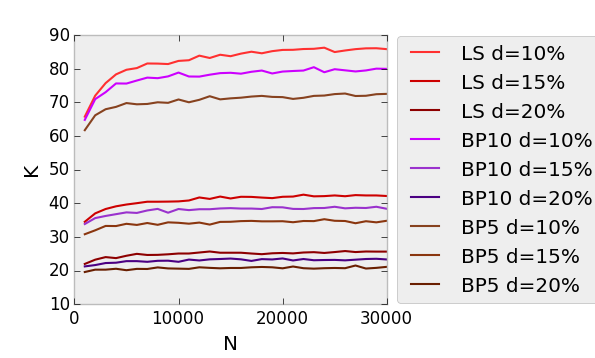
\includegraphics[width=0.9\linewidth]{Pictures/unif_ls_bp_k} 
    %\caption{$N=10$} 
    \label{fig:unif_ls_bp_k} 
    \vspace{4ex}
  \end{subfigure}%% 
  \begin{subfigure}[b]{0.5\linewidth}
    \centering
    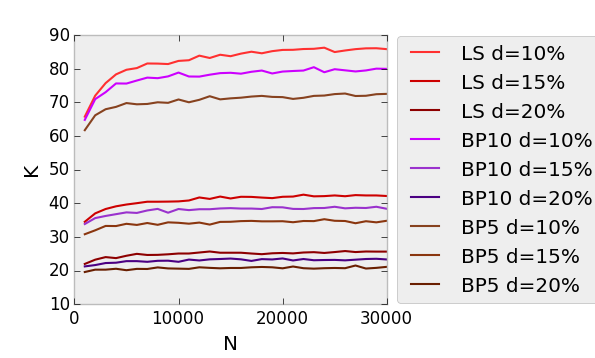
\includegraphics[width=0.9\linewidth]{Pictures/unif_ls_bp_k} 
    %\caption{$N=20$} 
    \label{fig:clus_ls_bp_k} 
    \vspace{4ex}
  \end{subfigure}
  \caption{Number $K$ of points for both two-phase filter algorithms on uniform inputs(left) and clustered inputs(right). The red lines represent the control group (line sweep), the purple lines represent the $10\%d$ first pass and the brown lines represent the $5\%d$ first pass for the two-phase algorithm.}
  \label{fig:ls_bp_k} 
\end{figure}

